\section{Untangling Size and Depth}
\seclabel{sizeconstancy}
Monocular cues for depth perception have been well-studied in psychology literature and there are two very important cues which emerge that tie object size and depth -  namely familiar size and relative size. Familiar size is governed by the fact that the visual angle subtended by an object decreases with distance from the observer and prior knowledge about the actual size of the object can be leveraged to obtain absolute depth of the object in the scene. Relative size, on the other hand, helps in explaining relative depths and sizes of objects - if we know that two objects are of similar sizes in the real world, the smaller object in the image appears farther. Another simple cue for depth perception arises due to perspective projection - an object further in the world appears higher on the image plane. Leveraging these three cues, we show that one can estimate real world object sizes from just images. In addition to object sizes, we also estimate a coarse viewpoint for each image in the form of the horizon and camera height. 

The main idea behind the algorithm is to exploit pairwise size relationships between instances of different object classes in images. As we will show below, given support points of objects on the ground and some rough estimate of object sizes, one can estimate the camera height and horizon position in the image - and as a result relative object depths. And in turn, given object heights in the image and relative depths, one can figure out the real world object scale ratios. Finally, exploiting these pairwise size evidences across images, we solve for absolute real world sizes (upto a common scale factor or the metric scale factor). Note that we use size and height interchangeably here as our notion of object size here actually refers to the object height.
% Perspective projection figure
\begin{figure}
  \centering
  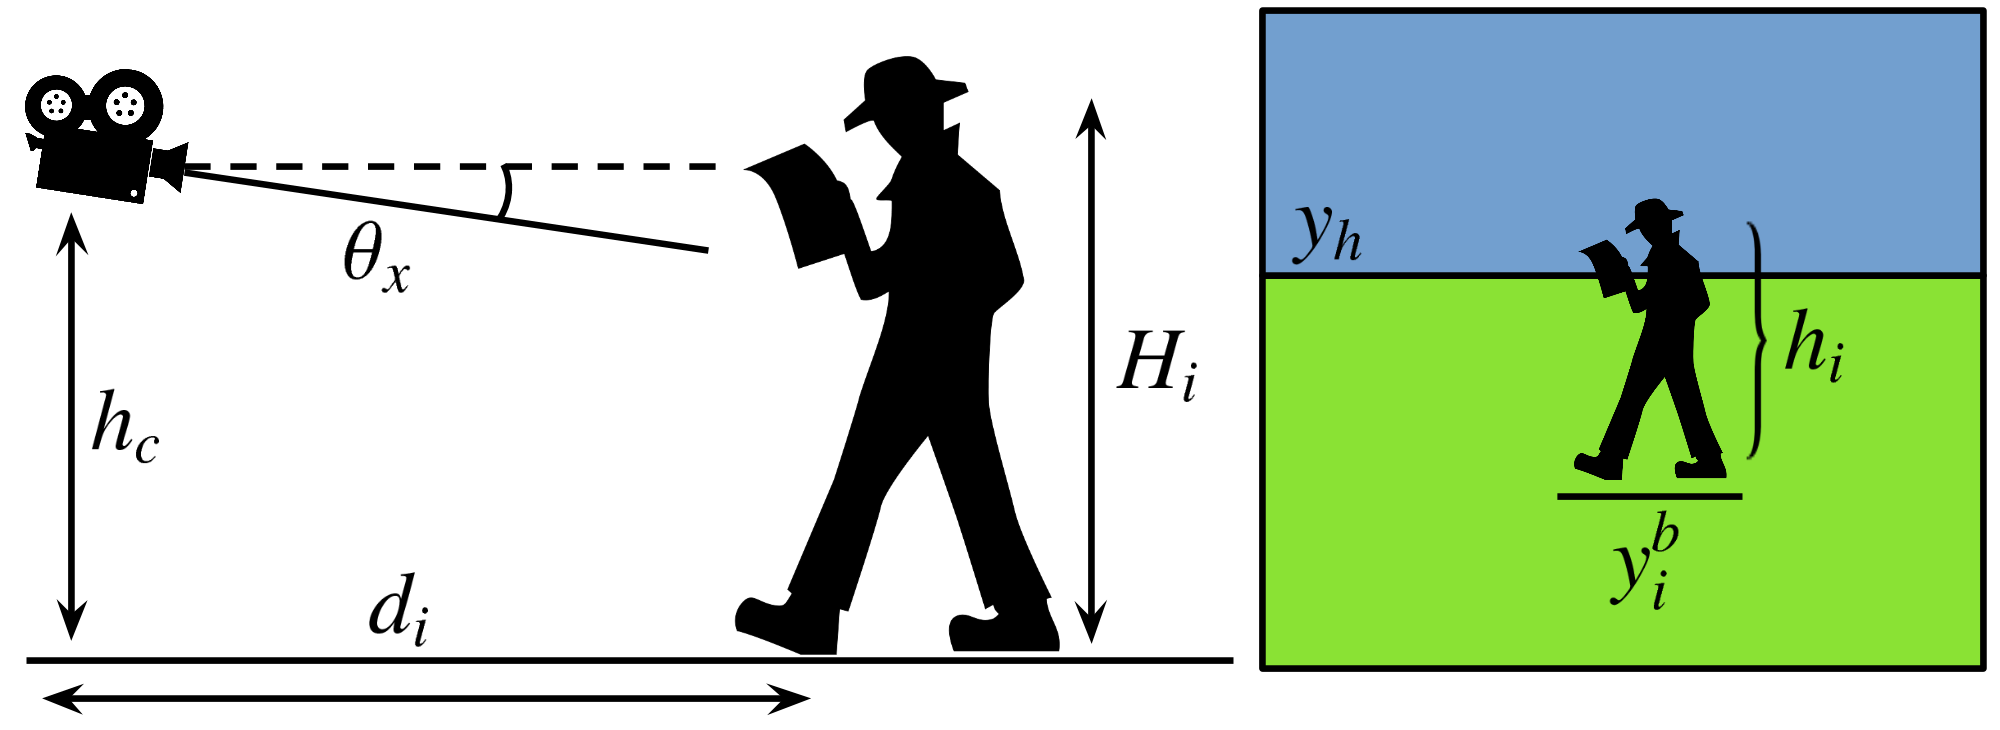
\includegraphics[width=\textwidth]{figures/amodal/Perspective.png}
  \caption{\figlabel{perspective} Toy example illustrating our camera model and parameters. Please refer to the text for detailed explanations. }
\end{figure}

\paragraph{Camera Model:} We use a simplified perspective camera model similar to Hoiem \etal~\cite{hoiem2008putting}. Let $f$ be the focal length of the camera, $\theta_x$ the camera tilt angle along the x-axis, $h_c$ the height of the camera, $y_h$ be the horizon position in the image, $y_i^b$ be the ground support point for the $i^{th}$ object in the image and $d_i$ be the distance of the $i^{th}$ object from the camera along the camera axis ($z$ axis). We assume that the images have been corrected for camera roll and all pixel co-ordinates are with respect to the optical center (assumed to be center of the image). \figref{perspective} provides a toy illustration of our model and parameters.

Assuming that the world frame is centered at the camera with its $y$ axis aligned with the ground, the projection of a world point $\mathbf{X} = (X_w,Y_w,Z_w)$ in the image in homogeneous co-ordinates is given by:
\bes
\begin{bmatrix}
x \\
y \\
1
\end{bmatrix} = \frac{1}{Z_w}
\begin{bmatrix}
f & 0 & 0\\
0 & f & 0\\
0 & 0 & 1
\end{bmatrix}
\begin{bmatrix}
1 & 0 & 0 & 0 \\
0 & \cos\theta_x & \sin\theta_x & 0 \\
0 & -\sin\theta_x & \cos\theta_x & 0 \\
\end{bmatrix}
\begin{bmatrix}
X_w \\
Y_w \\
Z_w \\
1
\end{bmatrix}
\ees
For a world point corresponding to the ground contact point of object $i$, given by $(X_w,-h,d_i)$, its corresponding $y$ co-ordinate in the image $y_i^b$ is given by:
$
y_i^b = f\frac{(-h_c/d_i + \tan\theta_x)}{1+(h_c/d_i)\tan\theta_x}
$
Under the assumption of the tilt angle being small ($\tan\theta_x \approx \theta_x$) and height of the camera being not too large compared to object distance ($h\theta_x \ll d_i$), our approximation is 
\be
\eqlabel{groundEq}
y_i^b = -\frac{fh_c}{d_i} + f\theta_x
\ee
Here $f\theta_x$ corresponds to the position of the horizon ($y_h$) in the image. Repeating the above calculation for the topmost point of the object and subtracting from \eqref{groundEq}, we obtain
\be 
\eqlabel{sizeEq}
h_i = \frac{fH_i}{d_i}
\ee
where $h_i$ refers to the height of the object in the image and $H_i$ is the real world height of the object.
Our model makes some simplifying assumptions about the scene namely, objects are assumed to rest on the same horizontal surface (here, the ground) and camera tilt is assumed to be small. We observe that for the purpose of size inference, these assumptions turn out to be reasonable and allow us to estimate heights of objects fairly robustly.

% Algorithm box for size estimation
\begin{algorithm}[h]
\caption{Object Size Estimation}
\begin{algorithmic}
\Initialize{Initial size estimates $\mathbf{H}$ and cluster assignments}
\While {not converged}
\ForAll{images $k \in $ Dataset }
\State $(h_c,y_h) \gets $ SolveLeastSquares($y_b,h,\mathbf{H}$)
\ForAll{pairs $(i,j)$ of objects in $k$}
\State $\frac{H_i}{H_j} \gets \frac{h_i}{h_j}\frac{y_j^b-y_h}{y_i^b-y_h}$\Comment{$(1)$}
\EndFor
\EndFor
\State $\log \mathbf{H} \gets$ least squares with pairwise constraints ($1$)
\State GMM cluster log scales ($\log \mathbf{H}$)
\State Reassign objects to clusters
\EndWhile
\end{algorithmic}
\label{alg:sizeEstimation}
\end{algorithm}

\paragraph{Inferring Object Sizes:} 
The important observation here is that the sizes of objects in an object category are not completely random - they potentially follow a multimodal distribution. For example, different subcategories of boats may represent the different modes of the size distribution. Given some initial sizes and size cluster estimates, our algorithm for size estimation (Algorithm \ref{alg:sizeEstimation}) works by estimating the horizon and camera height per image (by solving a least squares problem using \eqref{groundEq} and \eqref{sizeEq} for all the objects in an image). With the horizon and height estimated per image, we obtain pairwise height ratios $\frac{H_i}{H_j} = \frac{h_i}{h_j}\frac{y_j^b-y_h}{y_i^b-y_h}$ for each pair of objects in an image. We obtain multiple such hypotheses across the dataset which we use to solve a least squares problem for $\log \mathbf{H}$ - the log height for each size cluster. Finally, we cluster the log sizes obtained in the previous step to obtain new size clusters and iterate. Note that $\mathbf{H}$ refers to the vector with heights of various classes and $H_i$ refers to the real world size of the $i^{th}$ object.

This particular model is equivalent to solving a latent variable model where the latent variables are the cluster memberships of the instances, the estimated variables are heights corresponding to the size clusters and the horizon and camera height for each image. The loss function we try to minimize is the mean squared error between the ground contact point predicted by the model and the amodal bounding box. Finally, the log of the object heights are assumed to be a Gaussian mixture. This final assumption ties in elegantly with psychophysics studies which have found that our mental representation of object size (referred to as assumed size~\cite{ittelson1951size,baird1963retinal,epstein1963influence}) is proportional to the logarithm of the real world object size~\cite{konkle2011canonical}.

Our image evidences in the above procedure include the ground support points and heights for all the objects in the image. Note that amodal bounding boxes for objects provide us exactly this information. They account for occlusions and truncations and give us an estimate of the full extent of the object in the image. The above algorithm with occluded/truncated visible bounding boxes would fail miserably and we use our amodal bounding box predictor to first ``complete'' the bounding boxes for us before using our size inference algorithm to infer object heights.

\begin{figure}
  \centering
  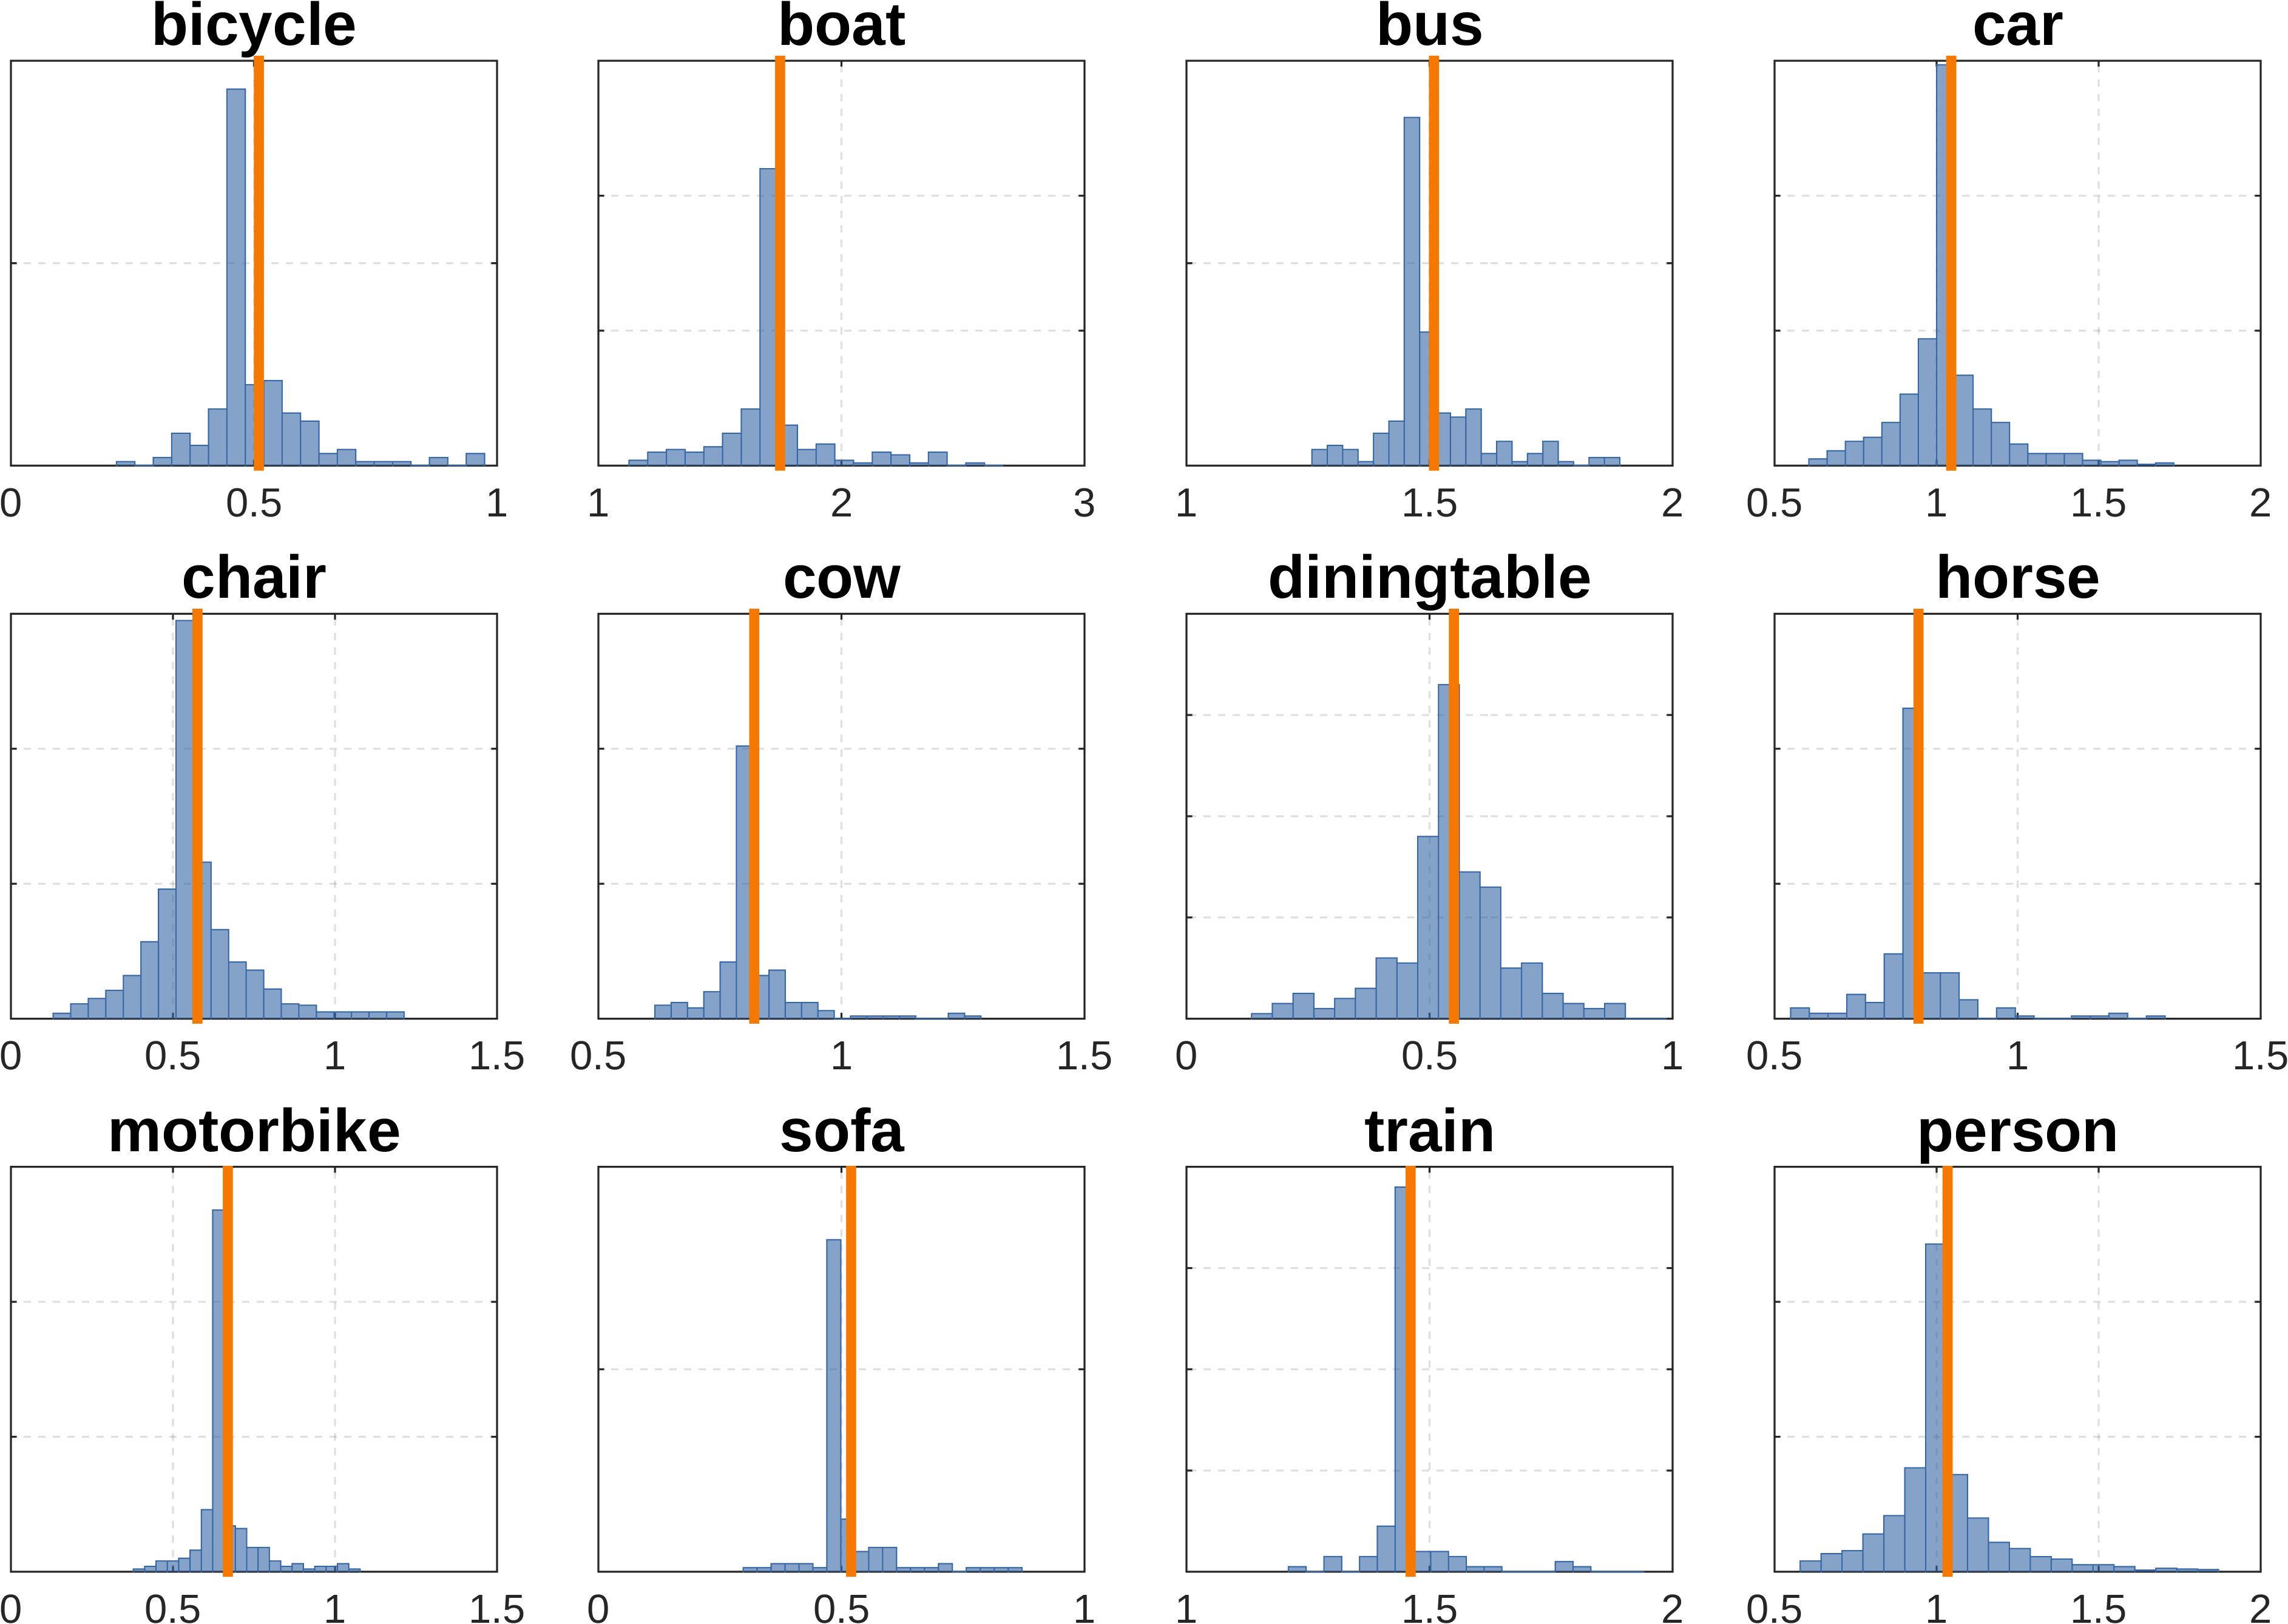
\includegraphics[width=\textwidth]{figures/amodal/size_PascalVal_pred.png}
  \caption{\figlabel{pascalSizes} Inferred log size distributions of 12 object categories on PASCAL VOC. We use our class agnostic amodal bounding box predictor to predict amodal boxes for all instances in VOC 2012 \textit{det-val} and use them with our object size estimation system to estimate size distributions for various categories. The plots above show distributions of the log size with the mean size being shown by the orange line.}
\end{figure}

\paragraph{Inferring Object Size Statistics on PASCAL VOC:} We used our size estimation system on PASCAL VOC to estimate size distributions of objects. First, we use our class agnostic amodal bounding box predictor on ground truth visible bounding boxes of all instances on VOC 2012 \textit{det-val} to ``upgrade'' them to amodal boxes. We initialize our system with a rough mean height for each object class obtained from internet sources (Wikipedia, databases of cars etc.) and run our size estimation algorithm on these predicted amodal boxes. \figref{pascalSizes} shows the distributions of log sizes of objects of various categories in PASCAL VOC. Most categories exhibit peaky distributions with classes such as ``boat'' and ``chair'' having longer tails owing to comparatively large intra class variation. Note that we experimented with using multiple size clusters per class for this experiment but the peaky, long tailed nature of these distributions meant that a single Gaussian capturing the log size distributions sufficed. In addition to inferring object sizes, we also infer the horizon position and height of the camera. The median height of the camera across the dataset was 1.4 metres (roughly the height at which people take images) and also exhibited a long tailed distribution (please refer to supplementary for details). Some examples of amodal bounding boxes estimated for all instances from visible bounding boxes and horizons are shown in \figref{resultFig}.


